Este apartado surge de la idea de analizar si es posible que un equipo alcance la cima del ranking, si los resultados hubieran sido distintos. Es decir, contamos con un schedule fijo, seleccionamos un equipo participante y tenemos la posibilidad de modificar los partidos perdidos del mismo a ganados. Interesa minimizar la cantidad de modificaciones de este estilo tal que el equipo seleccionado quede en primera posici\'on.

La estrategia que planteamos es la siguiente:

Sea EQUIPO* el equipo que interesa analizar

Calculamos los rankings con la entrada original.

Si ranking(EQUIPO*) es el m\'aximo retornamos la cantidad de iteraciones.

Si no, buscamos el equipo con m\'aximo ranking tal que EQUIPO* tenga alg\'un partido perdido que pueda ser modificado.

Se invierte el resultado y recalculamos los rankings con este cambio.

En caso de que sea imposible modificar un partido (ya se modificaron todos los posibles), retornamos la posicion final.

\textbf{Hip\'otesis:} Los equipos con m\'as derrotas deber\'an modificar m\'as resultados que los que tienen menos.

Estos fueron los standings finales de la temporada 2014-2015 de la NBA. A la derecha figura la cantidad de partidos que cada equipo deber\'ia ganar en vez de perder para quedar en la primera posici\'on seg\'un nuestro m\'etodo. \\

{\centering
\begin{tabular}{|c|c|c|c|}
\hline
Posici\'on & Equipo & Record & M\'inimo\\
\hline
1 & Golden State & 67-15 & 0 \\
\hline
2 & Atlanta & 60-22 & 8 \\
\hline
3 & Houston & 56-26 & 7 \\
\hline
4 & LA Clippers & 56-26 & 8 \\
\hline
5 & Memphis & 55-27 & 10 \\
\hline
6 & San Antonio & 55-27 & 11 \\
\hline
7 & Cleveland & 53-29 & 14 \\
\hline
8 & Portland & 51-31 & 13 \\
\hline
9 & Chicago & 50-32 & 18 \\
\hline
10 & Dallas & 50-32 & 13 \\
\hline
11 & Toronto & 49-33 & 18 \\
\hline
12 & Washington & 46-36 & 21 \\
\hline
13 & New Orleans & 45-37 & 19 \\
\hline
14 & Oklahoma City & 45-37 & 19 \\
\hline
15 & Milwaukee & 41-41 & 26 \\
\hline
16 & Boston & 40-42 & 27 \\
\hline
17 & Phoenix & 39-43 & 25 \\
\hline
18 & Brooklyn & 38-44 & 29 \\
\hline
19 & Indiana & 38-44 & 30 \\
\hline
20 & Utah & 38-44 & 26 \\
\hline
21 & Miami & 37-45 & 29 \\
\hline
22 & Charlotte & 33-49 & 33 \\
\hline
23 & Detroit & 32-50 & 35 \\
\hline
24 & Denver & 30-52 & 35 \\
\hline
25 & Sacramento & 29-53 & 34 \\
\hline
26 & Orlando & 25-57 & 41 \\
\hline
27 & LA Lakers & 21-61 & 44 \\
\hline
28 & Philadelphia & 18-64 & 48 \\
\hline
29 & New York & 17-65 & 50 \\
\hline
30 & Minnesota & 16-66 & 47 \\
\hline
\end{tabular} \\ }

Golden State qued\'o en primera posici\'on y por lo tanto requiere 0 partidos para tener el mejor ranking. No es algo sorprendente, pues adem\'as ganaron los Play-Off.

Para los dem\'as equipos, la estrategia indica que deben cambiar de perdidos a ganados, una cantidad de partidos tales que consigan una score final similar al que qued\'o en primera posici\'on.

Hay un caso interesante entre Portland, Chicago y Dallas, donde Chicago tiene el mismo record que Dallas, pero necesita 5 partidos m\'as que los otros dos equipos. Esto se debe al schedule de cada uno. Seguramente Chicago jug\'o pocos partidos frente a los equipos por encima de \'el, y probablemente haya ganado algunos. Mientras que Portland y Dallas deben haber jugado m\'as veces contras los mejor rankeados y perdido en la mayor\'ia de las oportunidades, con lo que una modificaci\'on en esos partidos, les significa un salto mayor en la escalada por el ranking.

Dada la observaci\'on sobre alcanzar el score del que finaliz\'o primero, probamos tambi\'en qu\'e sucede en el caso en que por ejemplo Golden State, ganara absolutamente todos los partidos. ¿Cu\'antos encuentros deber\'an ganar los dem\'as equipos para tener un ranking mejor?

Corrimos el algoritmo con este nuevo schedule y observamos que efectivamente
los resultados refuerzan las observaci\'on, pidi\'endole a cada equipo que ganara cerca de 80 partidos sobre 82 totales (ganar en vez de perder con Golden State para disminuir su ranking y ganarle a casi todos los dem\'as pues Golden State lo hab\'ia hecho).

Con respecto a la hip\'otesis planteada, podemos decir que a peor score, mayor cantidad de partidos necesarios que intercambiar, aunque est\'a intimamente ligado al schedule de cada equipo, especificamente a la cantidad de partidos jugados frente a los equipos mejor posicionados. Esto se ve porque la progresi\'on de scores es lineal (\ref{finalScores}), pero la de ratings zigzaguea, tendiendo a una parecerse a una funci\'on lineal con bajas repentinas (\ref{minimum})

\begin{figure}[h!]
  \begin{center}
	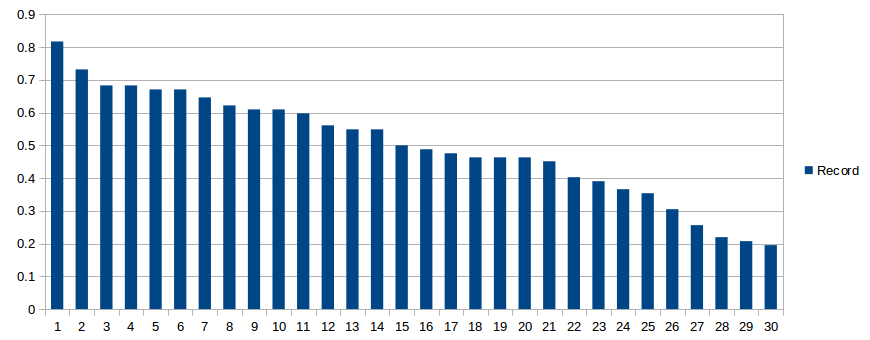
\includegraphics[scale=0.50]{imagenes/cualitative/greedy/scores.png}
	\caption{Scores finales}
	\label{finalScores}
  \end{center}
\end{figure}

\begin{figure}[h!]
  \begin{center}
	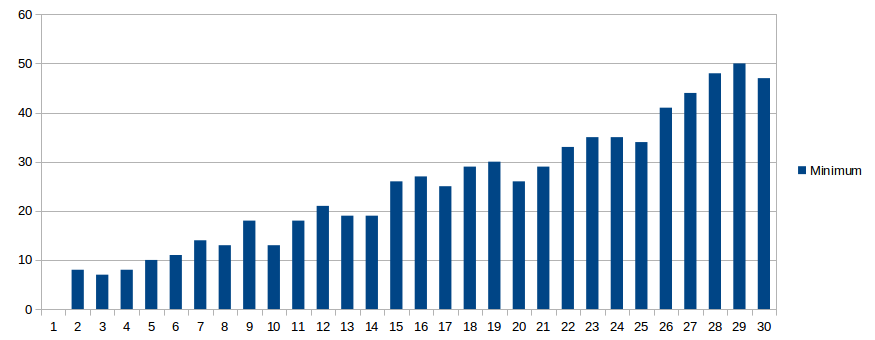
\includegraphics[scale=0.50]{imagenes/cualitative/greedy/minimum.png}
	\caption{N\'umero m\'inimo de partidos a modificar para alcanzar el primer puesto}
	\label{minimum}
  \end{center}
\end{figure}
